\documentclass[11pt,a4paper]{article}

% ---------------------------------------------------------------------------
% Packages
% ---------------------------------------------------------------------------
\usepackage[margin=2.4cm]{geometry}
\usepackage[utf8]{inputenc}
\usepackage[T1]{fontenc}
\usepackage{xcolor}
\usepackage{graphicx}
\usepackage{hyperref}
\usepackage{booktabs}
\usepackage{array}
\usepackage{longtable}
\usepackage{enumitem}
\usepackage{tikz}
\usepackage{titlesec}
\usepackage{fancyhdr}
\usepackage{amsmath}
\usepackage{tcolorbox}
\tcbuselibrary{skins,breakable}
\usetikzlibrary{arrows.meta, positioning, shapes.geometric, fit, backgrounds}

% ---------------------------------------------------------------------------
% Colors
% ---------------------------------------------------------------------------
\definecolor{c2ePrimary}{HTML}{0F172A}
\definecolor{c2eAccent}{HTML}{2563EB}
\definecolor{c2eAccent2}{HTML}{059669}
\definecolor{c2eWarn}{HTML}{D97706}
\definecolor{c2eGray}{HTML}{6B7280}
\definecolor{c2eBg}{HTML}{F8FAFC}

\hypersetup{
  colorlinks=true,
  linkcolor=c2eAccent,
  urlcolor=c2eAccent,
  citecolor=c2eAccent,
  pdftitle={Code2Edge -- Deployment with Proof},
  pdfauthor={Code2Edge Team},
  pdfsubject={IBM Bob 2.0 Hackathon Submission}
}

\titleformat{\section}
  {\normalfont\Large\bfseries\color{c2ePrimary}}
  {\thesection}{0.6em}{}[{\color{c2eAccent}\titlerule[1.2pt]}]
\titleformat{\subsection}
  {\normalfont\large\bfseries\color{c2ePrimary}}
  {\thesubsection}{0.6em}{}
\titleformat{\subsubsection}
  {\normalfont\bfseries\color{c2eAccent}}
  {\thesubsubsection}{0.6em}{}

\pagestyle{fancy}
\fancyhf{}
\renewcommand{\headrulewidth}{0.4pt}
\renewcommand{\footrulewidth}{0.4pt}
\fancyhead[L]{\small\color{c2eGray}Code2Edge --- Deployment with Proof}
\fancyhead[R]{\small\color{c2eGray}IBM Bob 2.0 Hackathon Submission}
\fancyfoot[C]{\small\color{c2eGray}\thepage}

\newtcolorbox{infobox}[1][]{
  breakable, enhanced, colback=c2eBg, colframe=c2eAccent,
  boxrule=0.6pt, arc=2pt, left=8pt, right=8pt, top=6pt, bottom=6pt,
  title={#1}, fonttitle=\bfseries\color{white},
  colbacktitle=c2eAccent, coltitle=white
}
\newtcolorbox{tagbox}{
  breakable, enhanced, colback=white, colframe=c2eGray!60,
  boxrule=0.5pt, arc=2pt, left=8pt, right=8pt, top=6pt, bottom=6pt
}

% ---------------------------------------------------------------------------
% Document
% ---------------------------------------------------------------------------
\begin{document}

% ===== Title page ============================================================
\begin{titlepage}
\centering
\vspace*{1.5cm}

{\Huge\bfseries\color{c2ePrimary} Code2Edge}\\[0.4cm]
{\Large\itshape\color{c2eAccent} Deployment with proof}\\[1.2cm]

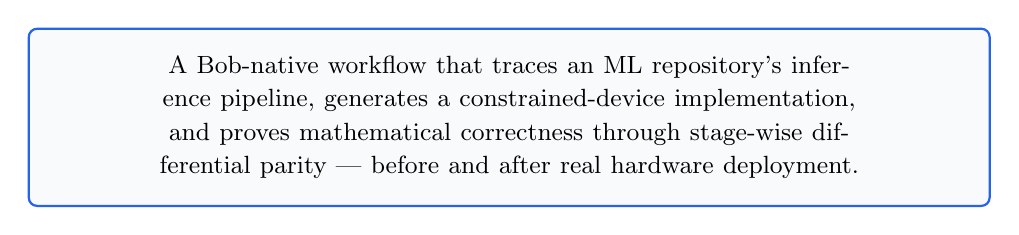
\begin{tikzpicture}
  \node[draw=c2eAccent, thick, rounded corners=3pt, fill=c2eBg,
        text width=11.5cm, align=center, inner sep=10pt]
  {\small A Bob-native workflow that traces an ML repository's inference
   pipeline, generates a constrained-device implementation, and proves
   mathematical correctness through stage-wise differential parity ---
   before and after real hardware deployment.};
\end{tikzpicture}

\vfill

{\large\bfseries IBM Bob 2.0 Hackathon (lablab.ai)}\\[0.2cm]
{\normalsize\color{c2eGray} 48-hour build}\\[1cm]

\begin{tabular}{ll}
\textbf{Target hardware:} & STM32U585 (ARM Cortex-M33) on Arduino UNO Q \\
\textbf{Reference workload:} & Keyword spotting, DS-CNN, 119{,}372 parameters \\
\textbf{Repository:} & \url{https://github.com/IndependentSalt69/Code2Edge}
\end{tabular}

\vspace{1.5cm}
{\small\color{c2eGray} This document was authored by Person C (Bob workflow,
MCP server, integration and submission) by reading the full repository
history, contracts, source, and evidence artifacts as of the commit noted
in Section~\ref{sec:results}.}

\end{titlepage}

\tableofcontents
\newpage

% ===============================================================================
\section{Basic Information}
\label{sec:basic}

\subsection{Project Title}
\textbf{Code2Edge}

\subsection{Short Description}
\begin{infobox}[Elevator pitch]
Code2Edge gives IBM Bob hardware awareness through an MCP server, so it can
trace an ML repository's audio pipeline, generate an equivalent C
implementation for a microcontroller, and \emph{prove} the two are
numerically equivalent --- stage by stage, on real hardware --- instead of
just hoping the ported code works.
\end{infobox}

\subsection{Long Description}

\subsubsection{The problem}
Deploying a PyTorch model to a microcontroller is not primarily a model
problem --- it is a \emph{pipeline} problem. A keyword-spotting model looks
simple: resample audio, window it, take an FFT, apply a Mel filterbank,
take a log, normalize, and feed the result to a small CNN. In practice this
chain is scattered across several files, with constants (window length, hop
size, FFT convention, epsilon values, per-channel normalization statistics)
buried in configuration that nobody reads twice. Reimplementing that chain
in C/C++ for an MCU is exactly where deployments silently break: a wrong
window size, an FFT power-vs-magnitude convention mismatch, or a log
epsilon that differs by one order of magnitude will still \emph{run} on the
device --- it will simply predict differently, and nothing in a
black-box ``does it boot'' test will tell you why.

Most edge-deployment tooling treats the on-device model as exactly that: a
black box, checked only by comparing final top-1 predictions. When accuracy
degrades after deployment, engineers have no visibility into \emph{which}
stage of the pipeline diverged.

\subsubsection{The approach}
Code2Edge attacks this with two ideas that reinforce each other:

\begin{enumerate}[leftmargin=1.4em]
  \item \textbf{Stage-wise differential parity, not black-box testing.} The
  same audio corpus is pushed through the Python/PyTorch reference
  pipeline and the generated C pipeline, and every intermediate tensor is
  compared: \texttt{max\_abs\_diff}, \texttt{mean\_abs\_diff}, cosine
  similarity, and (once the network runs) end-to-end prediction agreement
  and accuracy delta. When a stage's divergence exceeds its tolerance, the
  system reports the \emph{first} divergent stage and a deterministic
  diagnosis hint (e.g.\ ``shape mismatch at framing $\rightarrow$
  check hop length''), so debugging starts from evidence, not guesswork.
  \item \textbf{Bob as an orchestrator with hardware awareness, not a
  black-box code generator.} An MCP server exposes five hardware-aware
  tools --- \texttt{profile\_model}, \texttt{inspect\_pipeline},
  \texttt{check\_target}, \texttt{run\_parity\_test},
  \texttt{benchmark\_target} --- plus a small set of workflow tools
  (\texttt{start\_run}, \texttt{gate\_step}, \texttt{record\_approval}).
  Bob calls these tools to reason about the repository, the target's
  memory budget, and the parity results, and drives a fixed workflow:
  analysis $\rightarrow$ Edge Readiness Report $\rightarrow$ \emph{human
  approval checkpoint} $\rightarrow$ code generation $\rightarrow$ host
  parity gate (repair loop, capped at 3 attempts, then escalate to a
  human) $\rightarrow$ MCU build $\rightarrow$ device parity gate (same
  repair/escalate logic) $\rightarrow$ benchmark $\rightarrow$
  predicted-vs-measured report $\rightarrow$ git branch and pull request.
\end{enumerate}

\subsubsection{Why a human checkpoint}
Code2Edge deliberately puts a human in the loop \emph{before} any code
generation: Bob presents an Edge Readiness Report (does the model fit the
target's memory budget, what pipeline constants were found, what risks
exist) and waits for an explicit APPROVE or REJECT. This is enforced in
code (\texttt{workflow/approval.py}), not just in the workflow's
documentation --- generation cannot start without a recorded approval, and
a later approval overrides an earlier rejection for the same run.

\subsubsection{Reference workload}
Code2Edge is grounded in a real, trained model rather than a toy example:
a Depthwise-Separable CNN (DS-CNN, 119{,}372 parameters) trained for
12-class keyword spotting on the Google Speech Commands v0.02 dataset,
reaching 96.65\% test accuracy (\href{https://github.com/priyadeepjaiswal9c/tiny-kws}{\texttt{tiny-kws}}
by Priyadeep Jaiswal, vendored under \texttt{reference/tiny-kws/}, MIT
licensed, pinned to a specific upstream commit with SHA-256-verified file
integrity). The target is the STM32U585 MCU subsystem (ARM Cortex-M33,
160\,MHz, 786\,KB SRAM, 2\,MB Flash) on the Arduino UNO Q, whose Linux-side
Dragonwing QRB2210 MPU runs the Python reference and orchestration side.

\subsubsection{What actually got proven, honestly}
The team holds itself to the same standard the tool enforces on the
pipeline: every number in this submission is labeled as either \emph{real}
(measured or computed from a genuine artifact) or \emph{mock} (a
placeholder used when a hardware or data dependency was unavailable), and
the two are never blended silently. Section~\ref{sec:results} gives the
full breakdown; in short, host-side differential parity is \textbf{real
and fully passing} (500 samples, 4 pipeline stages, 2500/2500 stage
evaluations), and physical benchmarking is now \textbf{real and passing}
on the actual STM32U585 silicon (50/50 iterations correct). The one piece
still mocked in the latest end-to-end deployment run is device parity's
corpus-wide coverage --- a real single-fixture, single-stage on-device
comparison exists and passes, but not yet a full 500-sample sweep --- with
a hardware-validation guide checked into the deploy branch for completing
it.

\subsection{IBM Bob Usage Statement}
\begin{infobox}[How Bob was used]
Code2Edge is built \emph{for} Bob, not merely \emph{with} Bob: the MCP
server is the hardware-awareness layer that lets Bob reason about a
model repository and a memory-constrained target the way a human embedded
engineer would, and \texttt{workflow/WORKFLOW.md} is a literal,
step-by-step execution spec written for Bob to follow, including the exact
tool calls, the human-checkpoint protocol, and the retry/escalation policy
for both parity gates.
\end{infobox}

Concretely:
\begin{itemize}[leftmargin=1.4em]
  \item \textbf{MCP server as Bob's hardware senses.} Ten tools
  (\texttt{profile\_model}, \texttt{inspect\_pipeline}, \texttt{check\_target},
  \texttt{run\_parity\_test}, \texttt{benchmark\_target},
  \texttt{quantize\_model}, plus \texttt{start\_run}, \texttt{get\_run\_status},
  \texttt{gate\_step}, \texttt{record\_approval}) are registered in Bob's
  project MCP configuration (\texttt{.bob/mcp.json}) and were exercised
  directly through Bob during initial development (schema-validated mock
  responses, then real adapters as Person A and Person B's outputs became
  available).
  \item \textbf{Bob drove early repository and MCP scaffolding.} The
  project's initial local setup, repository survey, workspace scaffold,
  JSON-Schema tool contracts, and the first mock MCP server implementation
  were built in interactive Bob sessions; those sessions were exported and
  are checked into \texttt{bob\_sessions/} as part of this submission,
  alongside session transcripts for every later phase of the work.
  \item \textbf{The orchestration logic was authored generically for Bob to
  execute.} The parity-gate retry/escalation logic
  (\texttt{workflow/gates.py}) is written once and shared by both the host
  and device gates, enforcing a hard cap of 3 repair attempts before
  writing a structured escalation report for human debugging --- this cap
  is enforced in code, not left to the calling agent's discretion, so it
  behaves identically regardless of which agent (Bob, or a Bob-compatible
  execution environment) is driving it.
  \item \textbf{Transparency on execution environment.} During this 48-hour
  build the team could not confirm that the specific Bob build available
  supported defining a new project-level custom mode (only the three
  built-in Agent/Ask/Plan modes were discoverable in \texttt{.bob/}), so
  later phases of the same Bob-authored workflow were executed through an
  equivalent MCP-driven agent session following \texttt{workflow/WORKFLOW.md}
  verbatim, including its documented Fallback prompt for exactly this
  situation. Every one of those sessions is exported to
  \texttt{bob\_sessions/} with the same rigor as the native Bob exports, so
  the full decision trail --- tool calls, gate decisions, human
  approvals --- is auditable end to end.
\end{itemize}

\subsection{Technology \& Category Tags}

\begin{tagbox}
\textbf{Categories:} Agentic AI / Developer Tools \textbullet\ Edge AI \& TinyML
\textbullet\ Embedded Systems \textbullet\ MLOps \& Verification \textbullet\
Hardware-in-the-loop Testing
\end{tagbox}

\vspace{0.3cm}
\begin{longtable}{@{}p{3.6cm}p{10.8cm}@{}}
\toprule
\textbf{Category} & \textbf{Technologies} \\
\midrule
\endhead
Agent orchestration & IBM Bob (MCP client), Model Context Protocol (\texttt{mcp} Python SDK, FastMCP, stdio transport) \\
\addlinespace
Backend / tooling & Python 3.10+, \texttt{jsonschema} + \texttt{referencing} (Draft 2020-12), \texttt{pytest} + \texttt{pytest-asyncio}, \texttt{pyserial} \\
\addlinespace
ML / reference model & PyTorch, \texttt{torchaudio} (\texttt{MelSpectrogram}), Depthwise-Separable CNN (DS-CNN), Google Speech Commands v0.02 \\
\addlinespace
Edge code generation & Hand-verified C99 (Hann-windowed STFT, HTK Mel filterbank, log-compression, normalization), frozen int8 model array, TensorFlow Lite Micro / CMSIS-NN operator set \\
\addlinespace
Embedded target & STM32U585 (ARM Cortex-M33, TrustZone, FPU, Armv8-M DSP), Arduino UNO Q (Qualcomm Dragonwing QRB2210 host MPU), \texttt{arduino-cli} (\texttt{arduino:zephyr:unoq}), Zephyr RTOS \\
\addlinespace
Verification & Stage-wise differential parity (max/mean absolute error, cosine similarity), DWT-cycle-counter benchmarking, GCC linker-map memory accounting \\
\addlinespace
Version control \& CI hygiene & Git branch-per-owner workflow, Conventional Commits, JSON-Schema-gated contracts between team members, GitHub PRs merged as merge commits \\
\bottomrule
\end{longtable}

\newpage
% ===============================================================================
\section{System Architecture}
\label{sec:architecture}

Code2Edge is organized into three tiers, mirroring who owns what and how
data flows from a frozen research artifact to a proven on-device
deployment.

\begin{center}
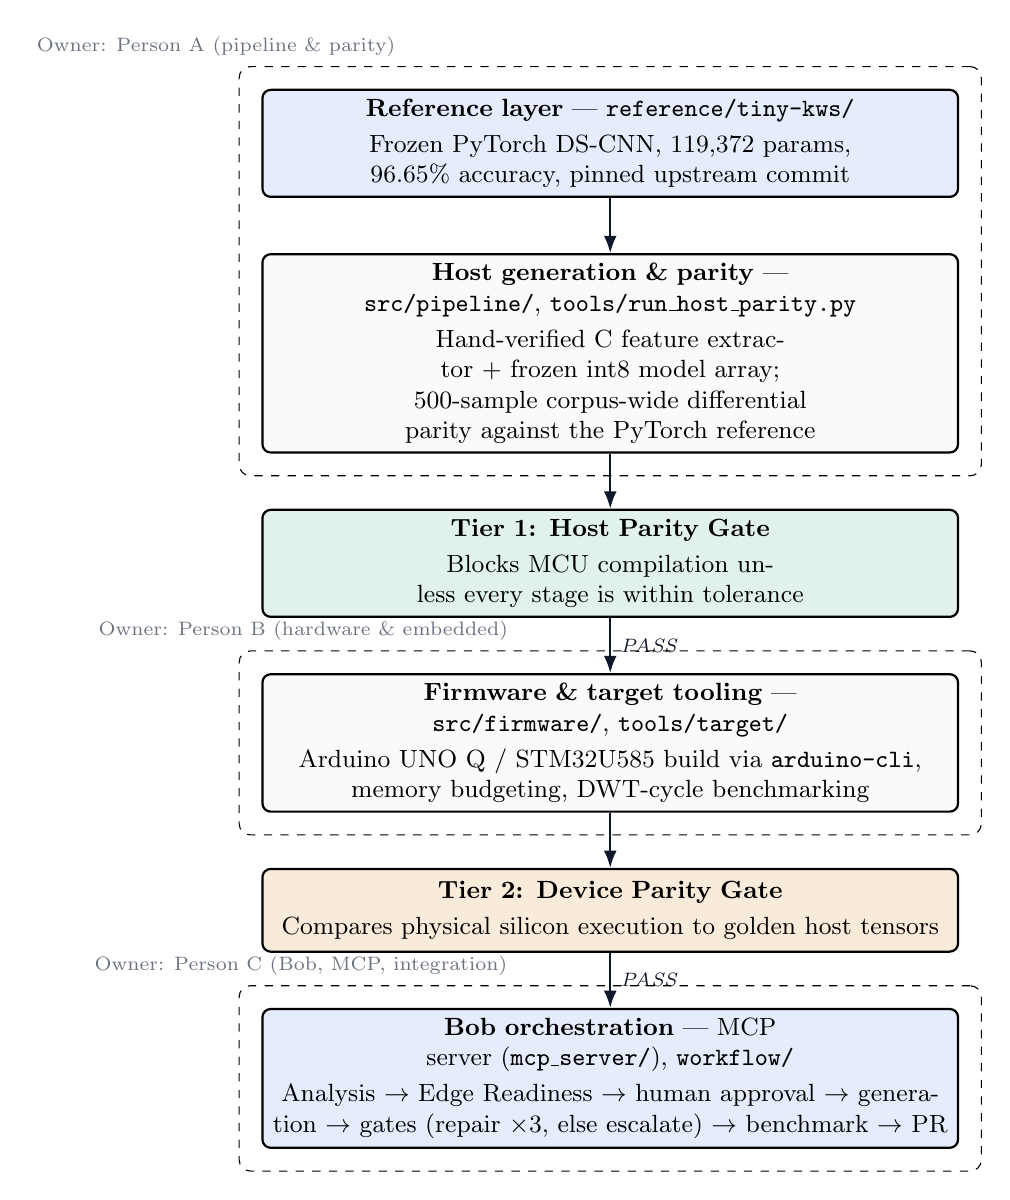
\begin{tikzpicture}[
  node distance=7mm and 14mm,
  box/.style={draw, thick, rounded corners=3pt, align=center, minimum height=1.05cm,
              text width=8.6cm, fill=c2eBg, font=\small},
  tier/.style={draw, dashed, rounded corners=4pt, inner sep=8pt},
  arr/.style={-{Latex[length=2.2mm]}, thick, color=c2ePrimary}
]

\node[box, fill=c2eAccent!12] (ref) {\textbf{Reference layer} --- \texttt{reference/tiny-kws/}\\[2pt]
  Frozen PyTorch DS-CNN, 119{,}372 params, 96.65\% accuracy, pinned upstream commit};

\node[box, below=of ref] (hostgen) {\textbf{Host generation \& parity} --- \texttt{src/pipeline/}, \texttt{tools/run\_host\_parity.py}\\[2pt]
  Hand-verified C feature extractor + frozen int8 model array;\\
  500-sample corpus-wide differential parity against the PyTorch reference};

\node[box, below=of hostgen, fill=c2eAccent2!12] (gate1) {\textbf{Tier 1: Host Parity Gate}\\[2pt]
  Blocks MCU compilation unless every stage is within tolerance};

\node[box, below=of gate1] (fw) {\textbf{Firmware \& target tooling} --- \texttt{src/firmware/}, \texttt{tools/target/}\\[2pt]
  Arduino UNO Q / STM32U585 build via \texttt{arduino-cli}, memory budgeting, DWT-cycle benchmarking};

\node[box, below=of fw, fill=c2eWarn!15] (gate2) {\textbf{Tier 2: Device Parity Gate}\\[2pt]
  Compares physical silicon execution to golden host tensors};

\node[box, below=of gate2, fill=c2eAccent!12] (bob) {\textbf{Bob orchestration} --- MCP server (\texttt{mcp\_server/}), \texttt{workflow/}\\[2pt]
  Analysis $\rightarrow$ Edge Readiness $\rightarrow$ human approval $\rightarrow$
  generation $\rightarrow$ gates (repair $\times$3, else escalate) $\rightarrow$
  benchmark $\rightarrow$ PR};

\draw[arr] (ref) -- (hostgen);
\draw[arr] (hostgen) -- (gate1);
\draw[arr] (gate1) -- node[right, font=\scriptsize\itshape] {PASS} (fw);
\draw[arr] (fw) -- (gate2);
\draw[arr] (gate2) -- node[right, font=\scriptsize\itshape] {PASS} (bob);

\node[tier, fit=(ref)(hostgen), label={[font=\scriptsize\color{c2eGray}]above left:Owner: Person A (pipeline \& parity)}] {};
\node[tier, fit=(fw), label={[font=\scriptsize\color{c2eGray}]above left:Owner: Person B (hardware \& embedded)}] {};
\node[tier, fit=(bob), label={[font=\scriptsize\color{c2eGray}]above left:Owner: Person C (Bob, MCP, integration)}] {};

\end{tikzpicture}
\end{center}

\subsection{Component map}

\begin{longtable}{@{}p{4.3cm}p{10.1cm}@{}}
\toprule
\textbf{Component} & \textbf{Responsibility} \\
\midrule
\endhead
\texttt{reference/tiny-kws/} & Immutable, pinned upstream research workload: weights, feature-extraction parameters, evaluation scripts. Governed by the upstream MIT license. \\
\addlinespace
\texttt{src/pipeline/} & Generated/verified C preprocessing (\texttt{feature\_extraction.c/.h}) and frozen int8 model array (\texttt{model\_data.c/.h}, 168.2\,KB, SHA-256 pinned). \\
\addlinespace
\texttt{src/firmware/} & Arduino/Zephyr application for the STM32U585, model runner integration. \\
\addlinespace
\texttt{tools/target/} & \texttt{check\_target} (memory-fit + toolchain readiness), \texttt{benchmark\_target} (physical DWT-cycle latency + linker-map memory), \texttt{run\_device\_parity} (on-device tensor comparison). \\
\addlinespace
\texttt{tools/run\_host\_parity.py} & Corpus-wide differential parity: compiles the C pipeline to a native shared library and diffs its output against frozen \texttt{.npy} reference tensors, stage by stage. \\
\addlinespace
\texttt{contracts/} & JSON Schemas (Draft 2020-12) for every MCP tool's input/output, shared and additively evolved across all three contributors. \\
\addlinespace
\texttt{mcp\_server/} & FastMCP server over stdio; per-tool mock/real mode switch via environment variables; schema validation on every response, mock or real. \\
\addlinespace
\texttt{workflow/} & \texttt{WORKFLOW.md} (the Bob execution spec), the run state machine, the generic parity gate with a hard-coded 3-attempt repair cap, and the human approval checkpoint. \\
\addlinespace
\texttt{evidence/}, \texttt{bob\_sessions/} & Committed proof artifacts (parity reports, benchmark evidence, per-sample CSVs) and exported agent session transcripts for every phase of the work. \\
\bottomrule
\end{longtable}

\newpage
% ===============================================================================
\section{Verification Methodology}
\label{sec:verification}

\subsection{Two-tier differential parity}
Code2Edge never compares only final predictions. Every intermediate tensor
in the pipeline is captured on the host reference, on the generated C
implementation (host-compiled), and --- for the second tier --- on the
physical MCU, and compared stage by stage.

\begin{center}
\resizebox{\textwidth}{!}{%
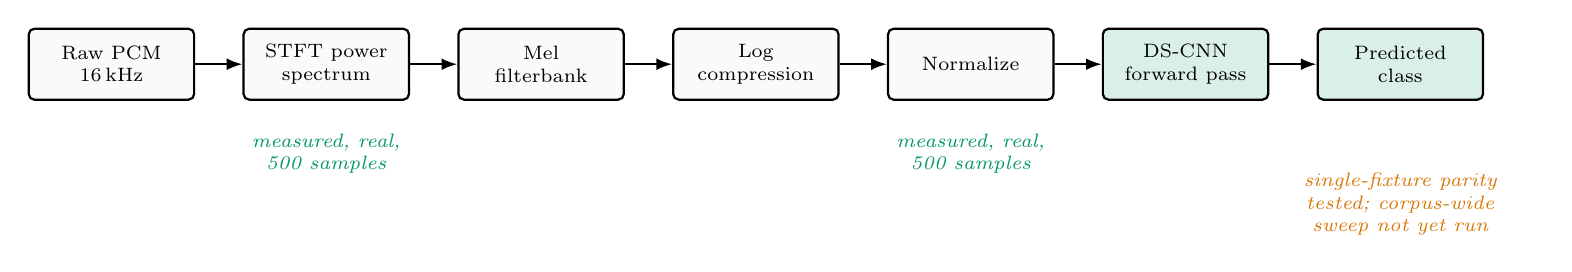
\begin{tikzpicture}[
  node distance=6mm,
  n/.style={draw, thick, rounded corners=2pt, fill=c2eBg, minimum width=2.1cm, minimum height=0.9cm, font=\scriptsize, align=center},
  arr/.style={-{Latex[length=2mm]}, thick}
]
\node[n] (input) {Raw PCM\\16\,kHz};
\node[n, right=of input] (fft) {STFT power\\spectrum};
\node[n, right=of fft] (mel) {Mel\\filterbank};
\node[n, right=of mel] (log) {Log\\compression};
\node[n, right=of log] (norm) {Normalize};
\node[n, right=of norm, fill=c2eAccent2!15] (net) {DS-CNN\\forward pass};
\node[n, right=of net, fill=c2eAccent2!15] (pred) {Predicted\\class};

\foreach \a/\b in {input/fft, fft/mel, mel/log, log/norm, norm/net, net/pred}
  \draw[arr] (\a) -- (\b);

\node[below=3mm of fft, font=\scriptsize\itshape\color{c2eAccent2}, text width=2.4cm, align=center] {measured, real, 500 samples};
\node[below=3mm of norm, font=\scriptsize\itshape\color{c2eAccent2}, text width=2.4cm, align=center] {measured, real, 500 samples};
\node[below=8mm of pred, font=\scriptsize\itshape\color{c2eWarn}, text width=3.4cm, align=center] {single-fixture parity tested; corpus-wide sweep not yet run};
\end{tikzpicture}%
}
\end{center}

\subsection{Stage tolerance matrix (design specification)}
\label{sec:tolerance}
\begin{longtable}{@{}p{1.0cm}p{3.3cm}p{2.5cm}p{2.9cm}p{2.9cm}@{}}
\toprule
\textbf{Stage} & \textbf{Name} & \textbf{Shape} & \textbf{Host tolerance} & \textbf{Device tolerance} \\
\midrule
\endhead
S0 & Raw audio PCM & $(16000,)$ & Exact & Exact \\
S1 & STFT power spectrum & $(1,201,101)$ & Rel.\ err.\ $\le 10^{-4}$ & Rel.\ err.\ $\le 10^{-3}$ \\
S1$'$ & Mel filterbank energy & $(1,64,101)$ & Rel.\ err.\ $\le 10^{-4}$ & Rel.\ err.\ $\le 10^{-3}$ \\
S2 & Log-Mel & $(1,1,64,101)$ & Rel.\ err.\ $\le 10^{-4}$ & Rel.\ err.\ $\le 10^{-3}$ \\
S3 & Normalized features & $(1,1,64,101)$ & Rel.\ err.\ $\le 10^{-4}$ & Rel.\ err.\ $\le 5\times10^{-3}$ \\
S4a--d & DS-CNN internal activations & varies & Rel.\ err.\ $\le 10^{-3}$ & Cosine sim.\ $\ge 0.99$ \\
S5 & Logits & $(1,12)$ & Abs.\ err.\ $\le 0.05$ & Abs.\ err.\ $\le 0.10$ \\
S6 & Predicted class & scalar & Exact match & Exact match \\
\bottomrule
\end{longtable}
\emph{Note: this is the full design tolerance matrix as specified in
\texttt{docs/validation.md}. Section~\ref{sec:results} reports which of
these were measured for real, at what sample-corpus scale, at the time of
this submission.}

\subsection{Repair loop}
When a stage exceeds tolerance, \texttt{gate\_step} returns one of three
decisions, computed --- and capped --- in code rather than left to agent
judgement:
\begin{itemize}[leftmargin=1.4em]
  \item \textbf{\texttt{continue}}: every stage passed; proceed to the next
  workflow step.
  \item \textbf{\texttt{repair}}: a stage failed and fewer than 3 attempts
  have been made; the agent is told the \texttt{focus\_stage} and a
  deterministic \texttt{repair\_hint}, and must retry.
  \item \textbf{\texttt{escalate}}: 3 attempts were exhausted (or the tool
  returned an unrecoverable error); a Markdown escalation report is written
  with every attempt's stage table and diagnosis hints, and the run stops
  for human debugging.
\end{itemize}

\newpage
% ===============================================================================
\section{Results}
\label{sec:results}

Every figure below is labeled \textbf{real} (measured, or computed from a
committed artifact) or \textbf{mock} (a placeholder, used only when a
hardware or data dependency was genuinely unavailable). The two are never
blended in a single reported number.

\subsection{Edge readiness (real)}
\begin{longtable}{@{}p{5.4cm}p{9.0cm}@{}}
\toprule
\textbf{Metric} & \textbf{Value} \\
\midrule
\endhead
Model & DS-CNN, 119{,}372 parameters (cross-checked exactly against the
  reference model's own reported parameter count) \\
Model flash footprint & 168.2\,KB (frozen int8 array, SHA-256 pinned) \\
Feature buffer & 25.3\,KB (64 Mel bins $\times$ 101 frames $\times$ 4 bytes) \\
Tensor arena (assumed) & 162.7\,KB \\
Total SRAM used & 188.0\,KB of 786\,KB budget --- \textbf{598\,KB headroom} \\
Total flash used & 168.2\,KB of 2048\,KB budget --- \textbf{$>$10$\times$ headroom} \\
Unsupported operators & None \\
\bottomrule
\end{longtable}

\subsection{Host differential parity (real)}
\begin{infobox}[Result: PASS]
500 audio samples $\times$ 4 real pipeline stages (STFT power spectrum,
Mel filterbank, log compression, normalization) = \textbf{2500/2500 stage
evaluations passed}, \texttt{first\_divergent\_stage: null}, on the first
attempt --- zero repairs needed.
\end{infobox}
Worst-case divergence across the entire corpus, by stage:
\begin{center}
\begin{tabular}{@{}lccc@{}}
\toprule
\textbf{Stage} & \textbf{Worst max.\ abs.\ diff} & \textbf{Worst cosine similarity} & \textbf{Tolerance} \\
\midrule
STFT power spectrum & $1.95\times10^{-3}$ & $0.999999999980$ & $10^{-2}$ \\
Mel filterbank & $9.77\times10^{-4}$ & $0.999999999981$ & $10^{-2}$ \\
Log compression & $7.83\times10^{-4}$ & $0.999999987766$ & $5\times10^{-3}$ \\
Normalization & $1.63\times10^{-4}$ & $0.999999999973$ & $10^{-3}$ \\
\bottomrule
\end{tabular}
\end{center}
This result is produced by compiling the same C source that ships in the
deploy branch to a native shared library and diffing its output against
frozen PyTorch reference tensors across the full 500-sample corpus
(\texttt{tools/run\_host\_parity.py} $\to$ \texttt{evidence/parity/host\_parity\_report.json}),
wired into \texttt{run\_parity\_test\_tool(gate="host")} so Bob reads it in
the same structured, stage-wise shape it would read a repair-loop failure
in.

\emph{Known limitation, disclosed rather than hidden:} the underlying host
harness currently hard-codes the source file it compiles and tests, so
this result verifies the deploy branch's copy of the pipeline \emph{by
identity} with the committed source, rather than independently
re-verifying an arbitrary generated copy in isolation --- logged as an open
item for the team.

\subsection{Device parity and physical benchmarking}
\label{sec:device-benchmark}
A single-fixture (\texttt{yes.wav}), single-stage (normalized features)
on-device comparison was run for real on physical STM32U585 silicon and
\textbf{passed} (cosine similarity $1.0000000950$, max.\ abs.\ error
$2.5\times10^{-5}$). This does not yet constitute a corpus-wide device
parity sweep (the 500-sample coverage the host side has) --- an open item
noted in \texttt{docs/interface-requests.md}.

The physical benchmark, by contrast, is now a full real DS-CNN inference
measurement on the actual board, not an infrastructure smoke test:

\begin{center}
\begin{tabular}{@{}lc@{}}
\toprule
\textbf{Metric} & \textbf{Measured value} \\
\midrule
Inference latency (mean, 50 runs) & 5026.2\,ms \\
Inference latency (min / max) & 5015.0\,ms / 5031.0\,ms \\
Inference latency (std.\ dev.) & 7.0\,ms \\
Clock cycles per inference & 804{,}196{,}284 \\
Flash used & 310{,}788\,B (14.8\% of 2\,MB) \\
SRAM used & 242{,}224\,B (30.1\% of 786\,KB) \\
Prediction correctness & 50/50 iterations --- logits, argmax and label all matched \\
\bottomrule
\end{tabular}
\end{center}

The multi-second latency is genuine and internally consistent
($804{,}196{,}284 \div 160\,\text{MHz} = 5.026\,\text{s}$, exactly matching
the reported mean) --- it reflects unaccelerated reference kernels rather
than CMSIS-NN SIMD dispatch, which \texttt{docs/hardware.md} already
flagged as not yet enabled at the time of writing. This is a real,
reportable performance finding, not a measurement error: the next
optimization target is enabling CMSIS-NN kernel dispatch for the
depthwise/pointwise convolutions, which should close most of that gap.

\subsection{The real deployment run}
\label{sec:run}
The full Bob workflow was executed end to end, producing a real git branch
and pull request:
\begin{itemize}[leftmargin=1.4em]
  \item Run analyzed the repository, produced an Edge Readiness Report, and
  \textbf{stopped for human approval} before any code was written.
  \item Generation copied the already-verified pipeline into an isolated
  \texttt{git worktree} (there is no separate code-authoring step; Bob's
  role is to orchestrate and prove, not to reinvent already-verified C++).
  \item Host parity gate: real, \textbf{PASS} on attempt 1, 0 repairs.
  \item Device parity and benchmark gates: mock at the time this specific
  run executed (no board was connected to the machine running it), clearly
  labeled, with a hardware validation guide committed alongside for
  completing them for real.
  \item A deploy branch was pushed and a pull request opened containing the
  generated code, both parity reports, the predicted-vs-measured table, and
  the hardware validation guide.
  \item \emph{Since that run}, the team has produced a real physical DS-CNN
  benchmark (Section~\ref{sec:device-benchmark}) --- the deploy branch's own
  benchmark artifact has not yet been re-run against it, so this submission
  reports it as a separate, current piece of evidence rather than silently
  back-filling the earlier PR.
\end{itemize}

\subsection{Engineering hygiene}
\begin{center}
\begin{tabular}{@{}lc@{}}
\toprule
\textbf{Metric} & \textbf{Value} \\
\midrule
Total commits (all branches) & 102 \\
Contributors & 4 \\
JSON-Schema contracts & 12 tools, all Draft 2020-12, 10/10 examples validating \\
Automated tests & 51 passing (\texttt{mcp\_server/} + \texttt{workflow/}) \\
Pull requests merged & 11, each with a merge commit (no history rewriting) \\
\bottomrule
\end{tabular}
\end{center}

\newpage
% ===============================================================================
\section{Team \& Attribution}

\subsection{Roles}
\begin{itemize}[leftmargin=1.4em]
  \item \textbf{Person A --- Pipeline \& Parity:} reference tensor dumping,
  the C feature-extraction implementation, and the host differential
  parity engine.
  \item \textbf{Person B --- Hardware \& Embedded:} STM32U585 toolchain,
  firmware integration, on-device parity, and the physical benchmark
  harness.
  \item \textbf{Person C --- Bob, MCP, Integration \& Submission:} the MCP
  server and tool contracts, the Bob workflow and its retry/escalation
  logic, git hygiene, the deploy branch/PR, and this submission.
\end{itemize}

\subsection{Third-party attribution}
\begin{itemize}[leftmargin=1.4em]
  \item \textbf{\href{https://github.com/priyadeepjaiswal9c/tiny-kws}{tiny-kws}},
  by Priyadeep Jaiswal --- used under the MIT License, vendored at a pinned
  upstream commit with SHA-256-verified file integrity.
  \item \textbf{Speech Commands Dataset} --- Pete Warden, \emph{``Speech
  Commands: A Dataset for Limited-Vocabulary Speech Recognition''}, 2018
  (CC-BY-4.0).
\end{itemize}

\end{document}
